% ----------------------------------------------------------------- %
%             The Speech Signal Processing Toolkit (SPTK)           %
%             developed by SPTK Working Group                       %
%             http://sp-tk.sourceforge.net/                         %
% ----------------------------------------------------------------- %
%                                                                   %
%  Copyright (c) 1984-2007  Tokyo Institute of Technology           %
%                           Interdisciplinary Graduate School of    %
%                           Science and Engineering                 %
%                                                                   %
%                1996-2012  Nagoya Institute of Technology          %
%                           Department of Computer Science          %
%                                                                   %
% All rights reserved.                                              %
%                                                                   %
% Redistribution and use in source and binary forms, with or        %
% without modification, are permitted provided that the following   %
% conditions are met:                                               %
%                                                                   %
% - Redistributions of source code must retain the above copyright  %
%   notice, this list of conditions and the following disclaimer.   %
% - Redistributions in binary form must reproduce the above         %
%   copyright notice, this list of conditions and the following     %
%   disclaimer in the documentation and/or other materials provided %
%   with the distribution.                                          %
% - Neither the name of the SPTK working group nor the names of its %
%   contributors may be used to endorse or promote products derived %
%   from this software without specific prior written permission.   %
%                                                                   %
% THIS SOFTWARE IS PROVIDED BY THE COPYRIGHT HOLDERS AND            %
% CONTRIBUTORS "AS IS" AND ANY EXPRESS OR IMPLIED WARRANTIES,       %
% INCLUDING, BUT NOT LIMITED TO, THE IMPLIED WARRANTIES OF          %
% MERCHANTABILITY AND FITNESS FOR A PARTICULAR PURPOSE ARE          %
% DISCLAIMED. IN NO EVENT SHALL THE COPYRIGHT OWNER OR CONTRIBUTORS %
% BE LIABLE FOR ANY DIRECT, INDIRECT, INCIDENTAL, SPECIAL,          %
% EXEMPLARY, OR CONSEQUENTIAL DAMAGES (INCLUDING, BUT NOT LIMITED   %
% TO, PROCUREMENT OF SUBSTITUTE GOODS OR SERVICES; LOSS OF USE,     %
% DATA, OR PROFITS; OR BUSINESS INTERRUPTION) HOWEVER CAUSED AND ON %
% ANY THEORY OF LIABILITY, WHETHER IN CONTRACT, STRICT LIABILITY,   %
% OR TORT (INCLUDING NEGLIGENCE OR OTHERWISE) ARISING IN ANY WAY    %
% OUT OF THE USE OF THIS SOFTWARE, EVEN IF ADVISED OF THE           %
% POSSIBILITY OF SUCH DAMAGE.                                       %
% ----------------------------------------------------------------- %
\hypertarget{lbg}{}
\name{lbg}{LBG algorithm for vector quantizer design}{vector quantization}

\begin{synopsis}
\item [lbg] [ --l $L$ ] [ --n $N$ ] [ --t $T$ ] [ --s $S$ ] [ --e $E$ ]
        [ --F $F$ ] [ --i $I$ ] [ --m $M$ ] [ --S $s$ ] 
\item [\ ~~~~~] [ --c $C$ ] [ --d $D$ ] [ --r $R$ ] [ {\em indexfile} ] $<$ {\em infile}
\end{synopsis}

\begin{qsection}{DESCRIPTION}
{\em lbg} uses the LBG algorithm to train a codebook 
from a sequence of vectors from {\em infile} (or standard input), 
sending the result to standard output.

The input sequence consists of $T$ float vectors $\bx$, 
each of size $L$
\begin{displaymath} 
\bx(0), \bx(1), \dots, \bx(T-1). 
\end{displaymath}
The result is a codebook consisting of $E$ float vectors, 
each of length $L$,
\begin{displaymath}
\bC_E =\{ \bc_E(0), \bc_E(1), \dots, \bc_E(E-1) \}, 
\end{displaymath}
generated by the following algorithm.

\begin{description}
\item[\bf step.0~~~]
When an initial codebook $\bC_S$ is not assigned,
the initial codebook is obtained from the whole collection of
training data as follows,
\begin{displaymath}
\bc_1(0) = \frac{1}{T} \sum_{n=0}^{T-1} \bx(n)
\end{displaymath}
and the initial codebook with $S = 1$ is $\bC_1 = \{ \bc_1(0) \}$.

\item[\bf step.1~~~]
From codebook $\bC_{S}$ obtain $\bC_{2S}$.
For this step, the normalized random vector of size $L$ and the splitting factor
$R$ are used as follows,
\begin{displaymath}
\bc_{2S}(n)= \begin{cases}
\;\;\bc_S(n) + R \cdot \bm{\mathrm{rnd}} & ( 0 \le n \le S-1 ) \\
\;\;\bc_S(n-S) - R \cdot \bm{\mathrm{rnd}} & ( S \le n \le 2S-1 )
\end{cases}
\end{displaymath}
and we make $D_0 = \infty$ , $k = 0$.

\item[\bf step.2~~~]
First, make sure that $k \le I$ where $I$ is the maximum iterations
number specified by --i option.
If it is true, proceed to the following steps.
If not, then go to {\bf step.4}.
The present codebook $\bC_{2S}$ is now applied
to the training vectors.
After that, the mean Euclidean distance $D_k$ is evaluated
from every training vector and their corresponding code vector.
If the following condition 
\begin{displaymath}
\left|\frac{D_{k-1}-D_{k}}{D_{k}}\right| < D
\end{displaymath}
is met, then go to {\bf step.4}.
If it is not met, then go to {\bf step.3}.
The steps 0, 1, and 2 are illustrated in figure \ref{fig:lbg_step0},
\ref{fig:lbg_step1}, and \ref{fig:lbg_step2}, respectivelly.

\begin{figure}[tbp]
\begin{minipage}{0.5\hsize}
\begin{center}
\fbox{
  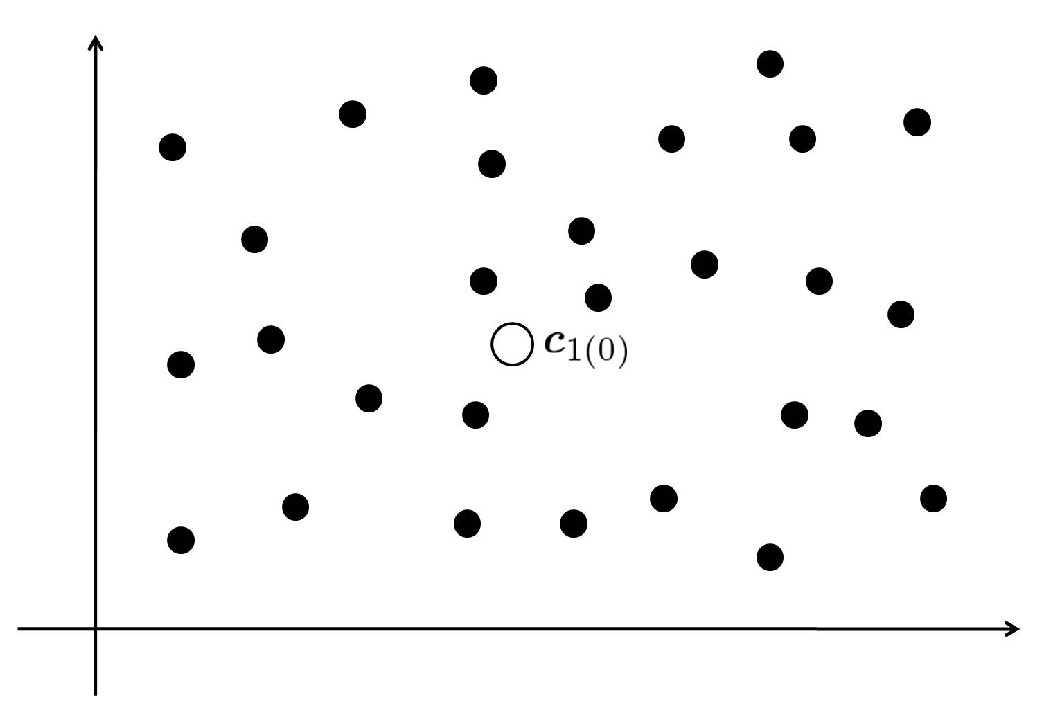
\includegraphics[width=5cm]{./fig/lbg_step0.eps}
}
\end{center}
\caption{{\bf step.0}: initialize codebook}
\label{fig:lbg_step0}
\end{minipage}
\begin{minipage}{0.5\hsize}
\begin{center}
\fbox{
  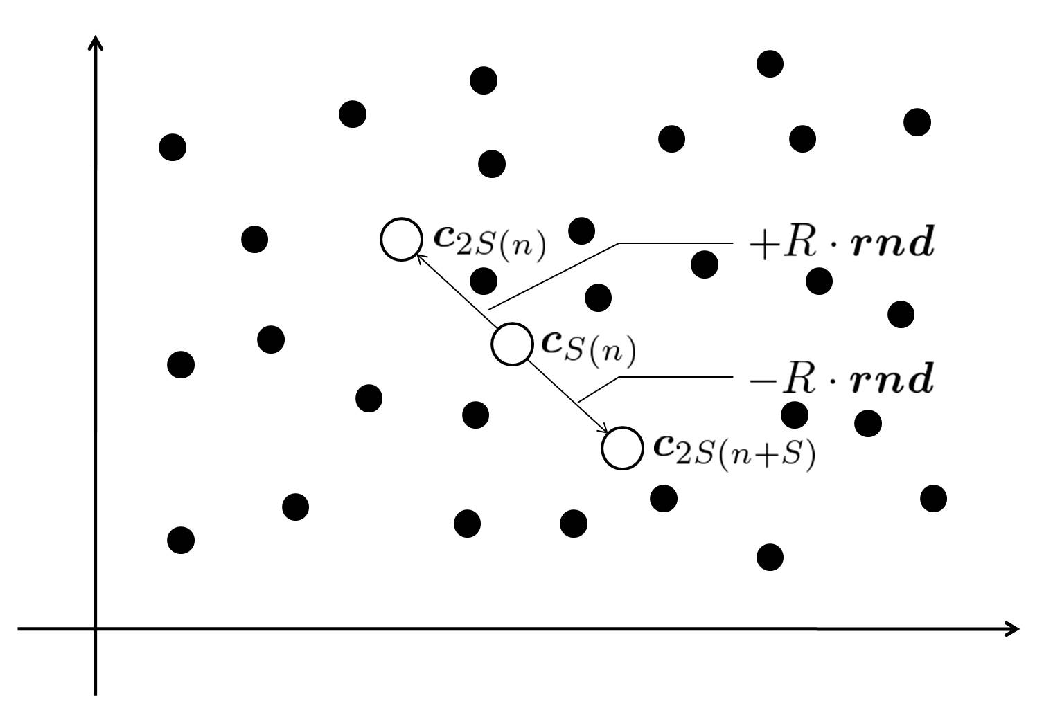
\includegraphics[width=5cm]{./fig/lbg_step1.eps}
}
\end{center}
\caption{{\bf step.1}: split codebook $\bC_{S}$ into $\bC_{2S}$}
\label{fig:lbg_step1}
\end{minipage}
\end{figure}
\begin{displaymath}
\left|\frac{D_{k-1}-D_{k}}{D_{k}}\right| < D
\end{displaymath}
\begin{figure}[tbp]
\begin{minipage}{0.5\hsize}
\begin{center}
\fbox{
  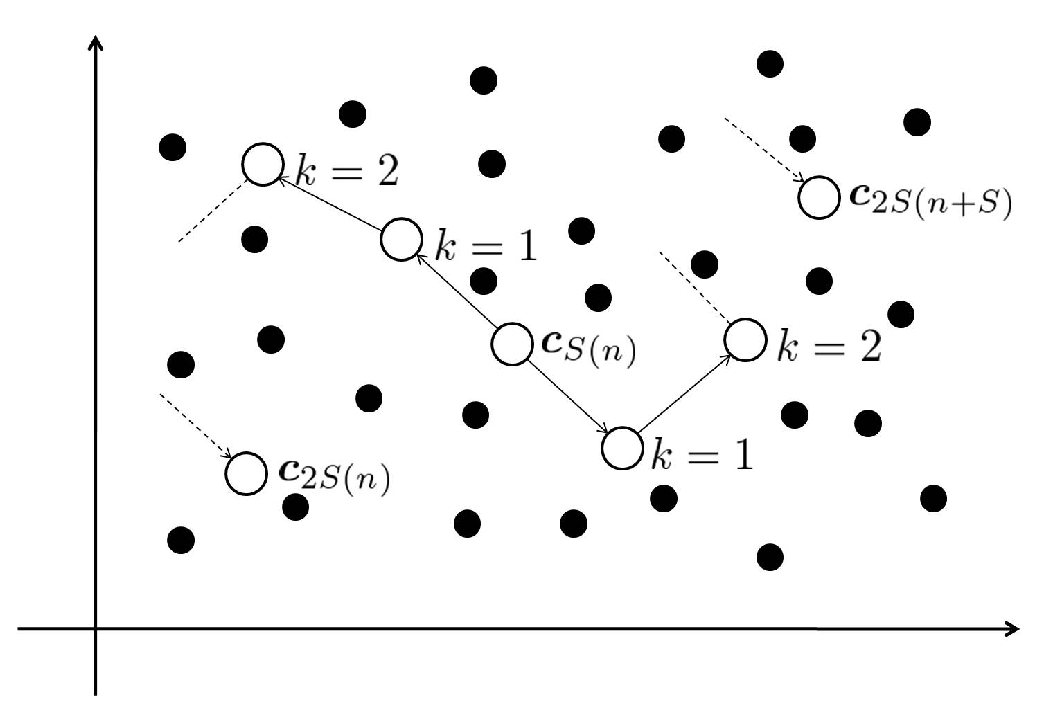
\includegraphics[width=5cm]{./fig/lbg_step2.eps}
}
\end{center}
\caption{{\bf step.2}: update codebook}
\label{fig:lbg_step2}
\end{minipage}
\end{figure}

\item[\bf step.3~~~]
Centroids are evaluated from the results obtained in {\bf step.2}.
Then, the codebook $\bC_{2S}$ is updated.
Also, if a cell has less than $M$ training vectors, then the corresponding
code vector is erased from the codebook,
and a new code vector is generated from either: 1) the code vector $\bc_{2S}(j)$  corresponding to the cell with more training vectors
, as follows.
\begin{displaymath}
\bc_{2S}(i) = \bc_{2S}(j) + R \cdot \bm{\mathrm{rnd}}
\end{displaymath}
Also, $\bc_{2S}(j)$ is modified as follows.
\begin{displaymath}
\bc_{2S}(j) = \bc_{2S}(j) - R \cdot \bm{\mathrm{rnd}}
\end{displaymath}
 2) the vector $\bp$, which internally divides
two centroids proportionally the number of training vectors for the cell.
They are split from the same parent centroid.
The vector $\bp$ is given by: 
\begin{displaymath}
\bp= \frac{n_{j}\bc_{2S}(i) + n_{i}\bc_{2S}(j)}{n_{i}+n_{j}},
\end{displaymath}
where $n_{i}$ and $n_{j}$ represent the number of training vectors for
the cells $\bc_{2S}(i) and \bc_{2S}(j)$, respectivelly.
The update method is as follows.
\begin{displaymath}
\bc_{2S}(i) = \bp + R \cdot \bm{\mathrm{rnd}},
\end{displaymath}
\begin{displaymath}
\bc_{2S}(j) = \bp- R \cdot \bm{\mathrm{rnd}}.
\end{displaymath}
If the number of traning vectors for the cell is less than $M$ when $k =
3$, the dividing vector $\bp$ and the update results are given as follows:

\begin{figure}[ht]
\setlength{\unitlength}{0.9mm}
\begin{center}
\begin{picture}(50,110)(20,0)
  \thicklines
  \put(60,105){\circle{10}}
  \put(49,105){\makebox(0,0){$k = 0$}}
  \put(80,108){\makebox(0,0){Parent centroid}} 
  \put(60,100){\vector(-2,-1){36}}
  \put(60,100){\vector(4,-3){28}}
  \put(24,79){\circle{6}}
  \put(88,76){\circle{6}}
  \put(15,79){\makebox(0,0){$k = 1$}}
  \put(97,76){\makebox(0,0){$k = 1$}}
  \put(24,76){\vector(-1,-2){15}}
  \put(88,73){\vector(3,-4){18}}
  \put(9,43){\circle{6}}
  \put(106,46){\circle{6}}
  \put(0,43){\makebox(0,0){$k = 2$}}
  \put(115,46){\makebox(0,0){$k = 2$}}
  \put(9,40){\vector(0,-1){15}}
  \put(106,43){\vector(-1,-3){5}}
  \put(9,22){\circle{6}}
  \put(101,25){\circle{6}}
  \put(0,22){\makebox(0,0){$k = 3$}}
  \put(110,25){\makebox(0,0){$k = 3$}}
  \put(9,15){\makebox(0,0){$\bc_{2S}(i)$}}
  \put(101,18){\makebox(0,0){$\bc_{2S}(j)$}}  
  \qbezier[90](12,22)(55,23)(98,25)
  \put(70,24){\circle*{20}}
  \thinlines
  \qbezier(12,22)(40,27)(67,24) 
  \qbezier(98,25)(85,27)(73,24)
  \put(70,24){\line(2,-1){24}}
  \put(94,12){\line(1,0){10}}
  \thicklines
  \put(40,27){\makebox(0,0)[b]{$n_i$}}
  \put(85,27){\makebox(0,0)[b]{$n_j$}}  
  \put(106,12){\makebox(0,0)[l]{dividing vector $\bp$}}
  \put(70,24){\vector(0,1){15}}
  \put(70,24){\vector(0,-1){15}}
  \put(70,42){\circle{6}}
  \put(70,6){\circle{6}}
  \put(69,34){\makebox(0,0)[r]{$+ R\cdot \bm{rnd}$}} 
  \put(69,14){\makebox(0,0)[r]{$- R\cdot \bm{rnd}$}}    
\end{picture}
\end{center}
\end{figure}

The type of split can be specified by the --c option.
After that, we assign $k=k+1$ and then go back to {\bf step.2}

\item[\bf step.4~~~]
If $2S = E$ then, end.
If not, then make $S$ = $2S$ and go back to {\bf step.1}.

\end{description}
\end{qsection}

\begin{options}
        \argm{l}{L}{length of vector}{26}
        \argm{n}{N}{order of vector}{L$-$1}
        \argm{t}{T}{number of training vector}{N/A}
        \argm{s}{S}{initial codebook size}{1}
        \argm{e}{E}{final codebook size}{256}
        \argm{F}{F}{initial codebook filename}{NULL}
        \argm{i}{I}{maximum number of iteration for centroid update}{1000} 
        \argm{m}{M}{minimum number of training vectors for each cell}{1}
        \argm{S}{s}{seed for normalized random vector}{1}
        \argm{c}{C}{type of exception procedure for centroid update \\
                    when the number of training vectors for the cell is less than $M$ \\
                    \begin{tabular}{ll} \\[-1ex]
                      $C=1$ & split the centroid with most training vectors\\
                      $C=2$ & split the vector which internally divide\\
                            & two centroids sharing the same parent centroid,\\
                            & in proportion to the number of training vectors for the cell.
                    \end{tabular}\\\hspace*{\fill}
                   }{1}
        \desc[1ex]{Usually, the options below do not need to be assigned.}
        \argm{d}{D}{end condition}{0.0001}
        \argm{r}{R}{splitting factor}{0.0001}
\end{options}

\begin{qsection}{EXAMPLE}
In the following example, a codebook of size 1024 is generated from
the 39-th order training vector {\em data.f} in float format.
It is also specified that the iterations for the centroid update are at most 100
 times, that each centroid contains at least 10 training vectors and that
 random vectors for the centroid update are generated with seed 5.
The output is written to {\em cbfile}.
\begin{quote}
\verb! lbg -n 39 -e 1024 -i 100 -m 10 -S 5 < data.f > cbfile!
\end{quote}
\end{qsection}

\begin{qsection}{SEE ALSO}
\hyperlink{vq}{vq},
\hyperlink{ivq}{ivq},
\hyperlink{msvq}{msvq}
\end{qsection}
